%% Generated by manuscript/build/build.py from main.src.md -- edit the source, not this file.
%% PLOS LaTeX template (journals.plos.org/ploscompbiol/s/latex), adapted for XeTeX/Tectonic.
\documentclass[10pt,letterpaper]{article}
\usepackage[top=0.85in,left=2.75in,footskip=0.75in]{geometry}
\usepackage{amsmath,amssymb}
\usepackage{changepage}
\usepackage{textcomp,marvosym}
\usepackage{cite}
\usepackage{nameref,hyperref}
\usepackage[right]{lineno}
\usepackage{iftex}
\usepackage[nopatch=eqnum]{microtype}
\ifpdftex\DisableLigatures[f]{encoding = *, family = * }\fi
\usepackage[table]{xcolor}
\definecolor{boxgray}{gray}{0.94}
\usepackage{array}
\usepackage{fvextra}
\usepackage{url}
\newcolumntype{+}{!{\vrule width 2pt}}
\newlength\savedwidth
\newcommand\thickcline[1]{%
  \noalign{\global\savedwidth\arrayrulewidth\global\arrayrulewidth 2pt}%
  \cline{#1}%
  \noalign{\vskip\arrayrulewidth}%
  \noalign{\global\arrayrulewidth\savedwidth}%
}
\newcommand\thickhline{\noalign{\global\savedwidth\arrayrulewidth\global\arrayrulewidth 2pt}%
\hline
\noalign{\global\arrayrulewidth\savedwidth}}
\raggedright
\setlength{\parindent}{0.5cm}
\textwidth 5.25in
\textheight 8.75in
\usepackage[aboveskip=1pt,labelfont=bf,labelsep=period,justification=raggedright,singlelinecheck=off]{caption}
\renewcommand{\figurename}{Fig}
\bibliographystyle{plos2025}
\makeatletter
\renewcommand{\@biblabel}[1]{\quad#1.}
\makeatother
\usepackage{lastpage,fancyhdr,graphicx}
\pagestyle{fancy}
\fancyhf{}
\rfoot{\thepage/\pageref{LastPage}}
\renewcommand{\headrulewidth}{0pt}
\renewcommand{\footrule}{\hrule height 2pt \vspace{2mm}}
\fancyheadoffset[L]{2.25in}
\fancyfootoffset[L]{2.25in}
\lfoot{\today}
%% PLOS asks for figures NOT to be embedded in the submission file; set \embedfiguresfalse for submission.
\newif\ifembedfigures
\embedfigurestrue
\begin{document}
\vspace*{0.2in}
\begin{flushleft}
{\Large
\textbf{BURROW: a fast protein pocket finder and ranker, designed, built and benchmarked end to end by AI agents}
}
\newline
\\\relax
[Author list, affiliations and corresponding author to be completed by the submitting authors]
\\
\bigskip
\textbf{Running title:} BURROW: agent-built pocket detection
\\
\bigskip
\textbf{AI-contribution statement.} All content of this article (study design, code, data curation, analyses, figures and text) was produced by AI agents: a principal-investigator agent and the sub-agents that it launched (Claude Code; Claude Opus 5.5 and Claude Sonnet 5.5; Anthropic). The human authors set up the computing environment, wrote the initial prompt, asked four follow-up questions, granted one time extension, requested this manuscript, and take responsibility for its submission. [The human authors will state here what they verified before submission.] See the box below, Methods and S2 Text.
\end{flushleft}

\bigskip
\noindent\fcolorbox{black}{boxgray}{\begin{minipage}{\dimexpr\linewidth-2\fboxsep-2\fboxrule\relax}\small

\textbf{How this work was produced.} This study is an experiment that tests whether AI agents can run a bioinformatics project from start to finish. AI agents did all of the work: the literature review, the design and its reviews, the pre-registration, the data curation, the code, the experiments, the statistical analyses, the figures and this text. The agents were a principal-investigator (PI) agent and the sub-agents that it launched for 30 roles: 25 during the project and 5 for the release repository and this manuscript (Claude Code with Claude Opus 5.5 and Claude Sonnet 5.5). They started from a single prompt. Approaches that did not work are described in S1 Text, and the prompt and all follow-up messages are reproduced verbatim in S2 Text. Human input was minimal. A human set up the compute environment and its data mounts and wrote the prompt. The same human later asked four follow-up questions (about multimers, GPU use, remaining ideas for speed and accuracy, and whether the work was finished), granted a 3--4 h time extension, and asked for this manuscript, pointing to a writing guide. The human did not write code, choose methods, select results or edit text. The Methods section (``Agent-based project execution'') describes the agent setup.

\end{minipage}}
\bigskip

\section*{Abstract}

Finding ligand-binding pockets in protein structures is a basic step in structure-based biology, and fast tools such as P2Rank remain hard to beat. We report BURROW, a pocket finder that uses no neural network, and how it was made: AI agents planned, built and benchmarked it from a single prompt with minimal human input. BURROW places candidate points on a 1 \AA{} grid, each standing for a small volume of space, and describes each point by ray-cast buriedness and by the chemistry of the first atom that each ray hits. Two gradient-boosted tree models score the points and rank the pockets. Claims and statistical tests were fixed before any test-set run, an independent agent audited the training data for leakage, and another recomputed the headline numbers. On LIGYSIS (2,775 chains, 6,721 non-redundant sites), BURROW's top-N+2 recall was 72.5\% (version 2, 9.1 pockets per chain), against 60.4\% for the best published method (fpocket+PRANK, 20.9 pockets per chain) and 52.6\% for our re-run of P2Rank. Version 1, frozen before any test predictions existed, reached 64.3\%. The difference between the versions comes from shorter output lists, which score better under the closest-pocket rule of the benchmark. Success within 4 \AA{} of ligand atoms was about 54\% in both versions, against 31.6\%. Most of the margin came from ion sites; on non-ion sites the gain was +3.0 to +3.5 points (+3.1 at 4 \AA{}). BURROW was non-inferior on HOLO4K and a temporal benchmark, and inconclusive on COACH420, apo/cryptic sites and dimer interfaces. An AlphaFold mode removed hallucinated pockets but did not beat a simple filter at pLDDT 70. Run as one process over 200 structures, BURROW took 142 ms per structure and P2Rank 209 ms; an optional fast preset took 48 ms. We list the goals that were not met.

\section*{Author summary}

Proteins bind small molecules in pockets on their surface, and finding these pockets is a first step in drug discovery and in understanding protein function. Many computer programs predict pockets, but fair comparisons between them are hard. Test proteins often resemble training proteins, benchmarks differ in what counts as a binding site, and the length of a program's output list can change its score. We asked whether AI agents, working from a single written instruction, could build a better pocket finder and test it honestly. A team of AI agents read the literature and wrote and reviewed a design. They also fixed their statistical tests in advance, built training data without overlap with the test proteins, and wrote and benchmarked the software. The resulting method, BURROW, finds more known binding sites than existing tools on a large benchmark and runs in about a tenth of a second per protein. The agents also showed where the advantage comes from: mostly metal-ion sites, and shorter output lists. They found no advantage on hidden (cryptic) pockets or on pockets between two protein chains. This single run shows what one agent-run project delivered and where human oversight would have helped.

\clearpage
\newgeometry{top=0.85in,left=1in,right=1in,footskip=0.75in}
\linenumbers

\section*{Introduction}

This article reports both a method and an experiment. The experiment asked whether AI agents can run a computational biology project end to end, from the literature review to a benchmarked tool and a written report. All design, code, analyses and text were produced by AI agents: one PI agent and the sub-agents that it launched, working from one prompt with minimal human input (see the box above, Methods and S2 Text). We report the method and results, and also how the agents worked, because the process affects how far the results can be trusted. In this article, ``we'' refers to the agent team.

The task was to build a fast pocket finder that beats existing methods such as P2Rank, generalises across protein families and to apo and AlphaFold structures, handles homo- and heterodimers, and runs on CPU and GPU. Geometric methods find concave regions from atom coordinates alone: LIGSITE counts protein--solvent--protein events along grid lines ~\cite{hendlich1997}, PocketPicker casts rays to measure buriedness ~\cite{weisel2007}, and fpocket clusters Voronoi alpha spheres ~\cite{leguilloux2009}. Knowledge-based methods learn which surface regions bind ligands: PRANK rescores fpocket pockets with a random forest on point features ~\cite{krivak2015}, and P2Rank scores points on the solvent-accessible surface, clusters the positive points and ranks the clusters ~\cite{krivak2018}. Deep-learning methods such as DeepPocket, PUResNet, GrASP, VN-EGNN and IF-SitePred use 3D convolutions, graph networks or embeddings from protein language models ~\cite{aggarwal2022,kandel2024,smith2024,sestak2025,carbery2024}.

Fair comparison is difficult. Utgés and Barton built LIGYSIS, a benchmark of 2,775 human protein chains whose binding sites are pooled across many PDB entries, and re-ran 13 methods under one protocol ~\cite{utges2024}. fpocket rescored by PRANK had the highest top-N+2 recall (60.4\%; P2Rank 51.9\%), and no deep-learning method beat it. fpocket's candidate list contained about 91\% of the sites and P2Rank's only 57\% ~\cite{utges2024}. We read this as evidence that the room for improvement lies in a candidate set with high recall and a ranking whose scores are comparable across proteins. COACH420 and HOLO4K are the legacy P2Rank test sets ~\cite{krivak2018,yang2013,schmidtke2010}, CryptoBench tests cryptic sites on apo structures ~\cite{skrhak2025}, and PocketWatch uses a temporal split on predicted structures ~\cite{portnoi2026}. Leakage between training and test proteins is a recurring problem ~\cite{skrhak2025,portnoi2026,durairaj2024}.

AlphaFold models add failure modes ~\cite{jumper2021,varadi2022}: low-confidence disordered regions can pack against the core and create pockets that do not exist. Proteome-wide pocket atlases therefore remove pockets whose mean pLDDT is below 70 ~\cite{carpenter2025,zillmer2025} (Zillmer and Walther also remove pockets with mean PAE above 10 \AA{}), and AF2BIND removes low-confidence segments ~\cite{gazizov2026}. We found no public benchmark of pocket prediction on homo- and heterodimers.

Here we describe BURROW (buriedness-driven ultra-fast ranking of pockets, with confidence awareness), its pre-registered benchmark against published methods, and where its apparent gains come from properties of the benchmark rather than of the method.

\section*{Results}

\subsection*{BURROW: high-recall candidates and a learned ranking}

Fig 1 shows the pipeline. BURROW keeps only protein atoms and places candidate points on a 1 \AA{} grid in the solvent shell; each point stands for a small volume of space, not a point on the surface. A cheap test based on LIGSITE ~\cite{hendlich1997} keeps buried points at full resolution and only a coarser 3 \AA{} sub-lattice of the rest, so that shallow sites stay in the pool. Extra candidates are placed where two or more protein atoms could coordinate a metal ion. Surface-point methods often miss such sites, and dedicated tools such as Metal3D also predict them ~\cite{durr2023}.

\begin{figure}[!h]
\ifembedfigures\centering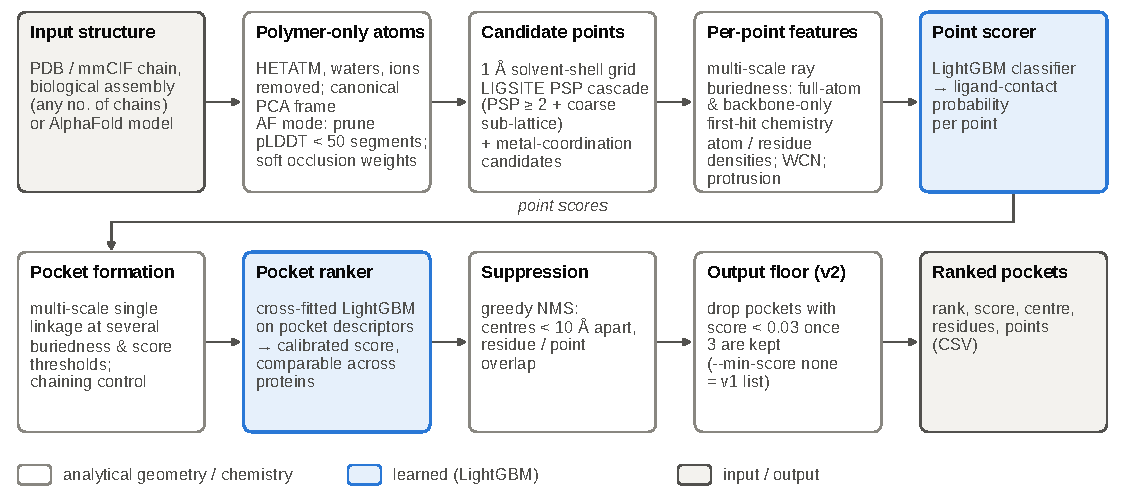
\includegraphics[width=\linewidth,height=0.55\textheight,keepaspectratio]{figures/fig1_pipeline.pdf}\fi
\caption{{\bf The BURROW pipeline.}
Top row: analytical geometry. Only protein atoms are kept (ligands, waters and ions are removed). In \texttt{--af-mode}, low-confidence segments (pLDDT \textless{} 50) are removed and atoms get soft occlusion weights, w = clip((pLDDT $-$ 40)/40, 0, 1). Candidate volume elements come from a 1 \AA{} solvent-shell grid that is filtered by a LIGSITE protein--solvent--protein (PSP) test, plus metal-coordination candidates. Each point is described by ray-cast buriedness at several ray lengths (through a full-atom grid and a backbone-only grid), first-hit chemistry, densities of atom and residue classes, weighted contact number (WCN) and protrusion. A LightGBM classifier scores the points. Bottom row: candidate pockets are formed by single linkage at several thresholds of buriedness and point score, with control of chaining. A LightGBM ranker that was trained on cross-fitted point scores ranks them, so that scores can be pooled across proteins. A pocket is suppressed if its centre lies within 10 \AA{} of a better-ranked pocket or if it overlaps one. The v2 output floor then drops pockets that score below 0.03 once three have been kept. Blue boxes are learned steps. Parameters are those of the final version (v2, default preset).}
\label{fig1_pipeline}
\end{figure}

Each point has 84 features. Rays cast through a full-atom grid and a backbone-only grid measure buriedness on several scales; the backbone-only grid is less sensitive to side-chain positions. For each ray, BURROW also records the chemical class of the first atom that the ray hits. We call this first-hit chemistry: a rough proxy for what a ligand at that point would contact and for the cost of desolvation. Other features are local atom and residue counts, the weighted contact number as a measure of flexibility ~\cite{lin2008}, protrusion ~\cite{krivak2018} and metal-coordination geometry.

A LightGBM classifier ~\cite{ke2017} scores the points, and BURROW forms pockets on several scales from buried and from high-scoring points. A second LightGBM model ranks the pockets. It is trained on cross-fitted point scores ~\cite{chernozhukov2018}, with a target that decreases with the distance to the nearest site. Both choices aim to make scores comparable across proteins; pooled precision (P1K, below) tests this, but we did not analyse calibration directly. Pockets within 10 \AA{} of a better-ranked pocket are suppressed. In the final version (v2), pockets that score below 0.03 are dropped once three have been kept (the output floor).

Two rankers share the features: \texttt{all}, trained on ion and non-ion sites, and \texttt{small}, trained on non-ion ligands to match COACH420, HOLO4K, CryptoBench and PocketWatch. The mapping to benchmarks was fixed before any results existed. Training sites came from BioLiP2 ~\cite{zhang2024}, built like LIGYSIS sites, with every chain similar to a test chain removed; about 38\% contain only ions. Table 1 credits the published ideas that BURROW builds on.

\begin{table}[!ht]
\begin{adjustwidth}{-0.0in}{0in}
\centering
\caption{{\bf Origins of BURROW's design choices.} Ideas taken from published work, and what BURROW changed. ``Agents'' marks choices that came from the agents' design reviews rather than from a single published source.}
\label{table_origins}
{\footnotesize
\begin{tabular}{p{3.1cm}p{5.3cm}p{6.3cm}}
\hline
\textbf{Design element} & \textbf{Source} & \textbf{What BURROW does} \\ \thickhline
Score points, cluster them, rank the clusters & P2Rank and PRANK ~\cite{krivak2018,krivak2015} & Same three-stage architecture. Points are volume elements on a grid rather than surface points. Gradient-boosted trees replace random forests. A separate pocket ranker is trained on cross-fitted point scores. \\ \hline
Candidate recall as the target & LIGYSIS analysis: fpocket's list contains about 91\% of sites, P2Rank's 57\% ~\cite{utges2024} & Own grid candidates reach 99.3\% maximum recall on LIGYSIS before the output floor (at 32.9 pockets per chain). \\ \hline
Protein--solvent--protein buriedness & LIGSITE ~\cite{hendlich1997,huang2006} & Used as a cheap first filter that decides which points are kept at full resolution. \\ \hline
Buriedness from ray casting, on several scales & PocketPicker ~\cite{weisel2007}; multi-scale buriedness in Ghecom ~\cite{kawabata2010} & Fibonacci rays at 6--24 \AA{} through a full-atom grid and a backbone+C$\beta$ grid (the latter tolerates side-chain changes). \\ \hline
Protrusion & P2Rank's most important feature ~\cite{krivak2018} & Kept as one feature among many. \\ \hline
Enclosure and polarity as druggability descriptors & SiteMap ~\cite{halgren2009}; fpocket druggability score ~\cite{schmidtke2010b} & First-hit chemistry: the chemical class of the first atom that each ray hits. \\ \hline
Weighted contact number as a flexibility measure & Lin et al. ~\cite{lin2008} & Mean weighted contact number around each point. \\ \hline
Cross-fitting of first-stage predictions & Double/debiased machine learning ~\cite{chernozhukov2018} & Ranker trained on out-of-fold point scores. \\ \hline
Site definition, redundancy rule, closest-pocket protocol, top-N+2 metric & LIGYSIS ~\cite{utges2024} & Training sites built the same way (fingerprint clustering, relative intersection, cut 0.5); metric and protocol ported and verified against the authors' code. \\ \hline
Relevant-ligand labels & BioLiP2 ~\cite{zhang2024} & Training labels, including metal ions. \\ \hline
Removal of low-confidence segments & AF2BIND (termini and internal runs of $\ge$ 7 residues with pLDDT \textless{} 50) ~\cite{gazizov2026} & Used unchanged as a fixed prior in \texttt{--af-mode}. \\ \hline
Pocket filter at mean pLDDT 70 & HOTPocket; Zillmer and Walther ~\cite{carpenter2025,zillmer2025} & Used as the control baseline that AlphaFold mode had to beat (it did not). \\ \hline
Leakage-aware and temporal evaluation & CryptoBench, PocketWatch, PLINDER ~\cite{skrhak2025,portnoi2026,durairaj2024} & Test union frozen before training; sequence filter with domain-level coverage; fold-disjoint ablation; independent audit. \\ \hline
Metal-site candidates; ions in the headline model & Agents (design review); metal-site location prediction, e.g. Metal3D ~\cite{durr2023} & Extra candidate points at metal-coordinating side chains; separate \texttt{all} and \texttt{small} rankers. \\ \hline
Pre-registration, Holm correction, cluster bootstrap & Agents (statistics review) ~\cite{holm1979} & Frozen claims, endpoints, margins and seeds before any test-set run. \\ \hline
\end{tabular}}
\end{adjustwidth}
\end{table}

``Analytical'' describes BURROW's candidates and features, not the source of its accuracy. Ranked without learning, the candidates reach 53.3\% top-N+2 recall on our development (dev) set, against 54.1\% for P2Rank. The gains below come from the learned scorer and ranker.

\subsection*{Benchmark design}

Table 2 lists the test benchmarks. We pre-registered three claims on LIGYSIS (family 1, tested in a fixed sequence) and six secondary endpoints with a non-inferiority margin of $-$2 points and Holm correction (family 2) ~\cite{holm1979}. Claims were frozen before any test-set run, and three amendments were each made before the relevant predictions existed. Our evaluation code first reproduced all 33 published LIGYSIS method variants to within 0.4 points (gate: 0.5), and our re-runs of P2Rank and fpocket+PRANK matched published values to within 2 points. Confidence intervals (CIs) are 95\% intervals from a paired bootstrap over clusters of chains with at least 30\% sequence identity.

\begin{table}[!ht]
\begin{adjustwidth}{-0.0in}{0in}
\centering
\caption{{\bf Test benchmarks.} All benchmarks were frozen before any BURROW test prediction. Endpoint codes refer to the pre-registered claims (C, family 1; O, family 2). Sites and units are scored sites and cluster-bootstrap units.}
\label{table_benchmarks}
{\footnotesize
\begin{tabular}{p{3.0cm}p{4.2cm}p{3.0cm}p{4.0cm}}
\hline
\textbf{Benchmark} & \textbf{Endpoint} & \textbf{Size} & \textbf{Input} \\ \thickhline
LIGYSIS ~\cite{utges2024} (C1, C1-strict, C2) & Top-N+2 recall at DCC $\le$ 12 \AA{} (closest pocket); DCA $\le$ 4 \AA{}; P1K & 2,775 chains, 6,721 non-redundant sites of 6,882 (6,387 with ligand atoms) & Authors' ligand-free representative chains \\ \hline
LIGYSIS without ions (descriptive) & As above & 2,003 chains, 4,141 sites & As above \\ \hline
COACH420, HOLO4K (mlig) ~\cite{krivak2018} (O2a, O2b) & DCA $\le$ 4 \AA{}, top-n, P2Rank rules & 379 and 6,874 ligands & P2Rank dataset files \\ \hline
PocketWatch test ~\cite{portnoi2026} (O3) & Top-N+2 at DCC $\le$ 12 \AA{}, authors' mask & 1,566 structures, 1,573 sites & Authors' predicted structures, \texttt{--af-mode} (no effect: no pLDDT) \\ \hline
CryptoBench test ~\cite{skrhak2025} (O4) & Top-N+2 at DCC $\le$ 12 \AA{} to the site centre on the apo structure & 222 apo structures, 270 sites & Apo structures \\ \hline
AlphaFold set, built here (O5) & Top-N+2 at DCC $\le$ 12 \AA{} & 2,526 AFDB v6 human models, 6,502 sites & Full-length models, \texttt{--af-mode} \\ \hline
Dimer set, built here (O6) & Interface top-N+2 at DCC $\le$ 12 \AA{} & 400 assemblies, 807 unique sites (243 at interfaces) & PDB assembly 1 \\ \hline
\end{tabular}}
\end{adjustwidth}
\end{table}

Two versions were scored. Version 1 (v1) output the full suppressed list of up to 50 pockets; version 2 (v2) added the output floor. v2 was chosen on dev data before any v1 test score was computed, but 70 minutes after the files with the v1 test predictions had been written. The pre-registered claims hold for v1 alone.

\subsection*{LIGYSIS: pre-registered claims pass for both versions}

Family 1 passed for both versions, all three seeds and both comparators (Fig 2, Fig 3A, Table 3). For v2, top-N+2 recall at a centre-to-centre distance (DCC) of at most 12 \AA{} was 72.0--72.5\% across seeds (72.5\% for seed 0), against 60.4\% for the published fpocket+PRANK predictions, on the 6,721 non-redundant sites (of 6,882) left by the LIGYSIS redundancy filter. The smallest difference was +11.6 points (lowest CI bound 9.4). v1 reached 64.3--64.9\% (smallest difference +3.9 [2.0, 6.0]). Our re-run of P2Rank 2.5.1 reached 52.6\% (published: 51.9\%).

\begin{figure}[!h]
\ifembedfigures\centering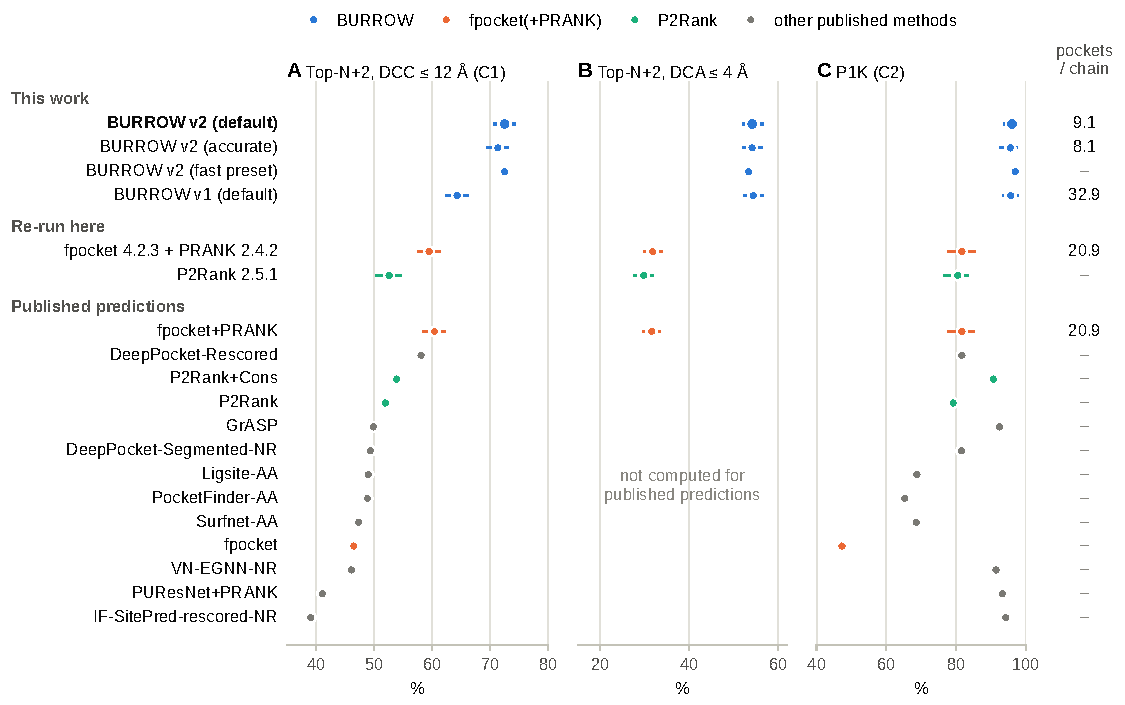
\includegraphics[width=\linewidth,height=0.55\textheight,keepaspectratio]{figures/fig2_ligysis.pdf}\fi
\caption{{\bf Pocket prediction on the LIGYSIS test set (2,775 chains, 6,721 binding sites).}
(A) Top-N+2 success: a site counts as found when the pocket closest to its centre is within 12 \AA{} (DCC) and has a rank of N+2 or better, where N is the number of sites on the chain (pre-registered endpoint C1). (B) The same with a stricter criterion for a hit: distance to any ligand atom (DCA) $\le$ 4 \AA{} (6,387 sites with ligand atoms; C1-strict). (C) Pooled precision P1K (endpoint C2): the share of true positives among the 1,000 highest-scoring pockets pooled over all chains. Right column: mean number of pockets that each method outputs per chain. Because the closest-pocket rule gives less credit to long output lists, top-N+2 must be read together with list length (see Fig 4). Points: seed 0 for BURROW. Bars: 95\% paired cluster-bootstrap CIs (30\% sequence clusters, 1,687 units, 1,000 resamples), shown where a CI was computed. ``Re-run here'': P2Rank 2.5.1 and fpocket 4.2.3 + PRANK 2.4.2, run on identical inputs. ``Published predictions'': the LIGYSIS authors' per-chain predictions, scored with our evaluation code, which reproduces their published numbers to within 0.4 points (gate: 0.5) for all 33 method variants. For these, except fpocket+PRANK (the C1 comparator), no CIs or pocket counts were computed, and chains without predictions count as misses. The fast preset was not pre-registered (descriptive).}
\label{fig2_ligysis}
\end{figure}

In C1-strict, a site counts as found only if the pocket closest to its ligand atoms lies within 4 \AA{} of them (DCA $\le$ 4 \AA{}) and has a rank of N+2 or better. BURROW v2 reached 54.0--54.2\%, against 31.6\% for fpocket+PRANK and 29.8\% for P2Rank. Pooled precision of the top 1,000 pockets (P1K) was 96.1--96.9\% against 81.7\%. P1K was pre-registered as non-inferiority; its CI [10.2, 19.0] also excludes zero. The best published P1K (94.3\%, a rescored IF-SitePred variant) is 1.8 points lower; we did not test that difference. An independent agent recomputed all headline numbers without project code, using the LIGYSIS authors' code for C1; all matched to within 0.2 points.

\begin{table}[!ht]
\begin{adjustwidth}{-0.0in}{0in}
\centering
\caption{{\bf Pre-registered test results (seed 0).} Comparator values are percentages; $\Delta$ is BURROW minus the comparator in percentage points, with 95\% paired cluster-bootstrap CIs. Family 1 comparator: published fpocket+PRANK predictions. Family 2 comparator: the better of P2Rank 2.5.1 and fpocket+PRANK on identical inputs (P2Rank's AlphaFold configuration for O3 and O5). Seeds 1 and 2 give the same decisions as seed 0 in both versions. The O4 point estimate varies most across seeds (v2: $-$2.6 to +1.1).}
\label{table_prereg}
{\footnotesize
\begin{tabular}{p{1.4cm}p{2.8cm}p{1.6cm}p{2.3cm}p{1.8cm}p{2.3cm}p{1.8cm}}
\hline
\textbf{Endpoint} & \textbf{Benchmark and metric} & \textbf{Comparator} & \textbf{v1 $\Delta$ [CI]} & \textbf{v1 decision} & \textbf{v2 $\Delta$ [CI]} & \textbf{v2 decision} \\ \thickhline
C1 & LIGYSIS top-N+2 (DCC 12 \AA{}) & 60.4 & +3.9 [2.0, 6.0] & pass & +12.1 [9.9, 14.2] & pass \\ \hline
C1-strict & LIGYSIS top-N+2 (DCA 4 \AA{}) & 31.6 & +22.9 [20.2, 25.9] & pass & +22.6 [20.0, 25.5] & pass \\ \hline
C2 & LIGYSIS P1K & 81.7 & +14.0 [10.1, 18.6] & pass (CI \textgreater{} 0) & +14.4 [10.2, 19.0] & pass (CI \textgreater{} 0) \\ \hline
O2a & COACH420 DCA4 top-n & 69.4 & +2.4 [$-$2.7, 7.1] & inconclusive & +1.6 [$-$3.0, 5.8] & inconclusive \\ \hline
O2b & HOLO4K DCA4 top-n & 76.6 & +1.8 [$-$1.0, 4.4] & non-inferior & +1.6 [$-$1.2, 4.3] & non-inferior \\ \hline
O3 & PocketWatch top-N+2 & 75.8 & $-$2.7 [$-$4.9, $-$0.5] & inconclusive & +0.8 [$-$1.4, 2.9] & non-inferior \\ \hline
O4 & CryptoBench apo top-N+2 & 71.9 & $-$5.2 [$-$11.1, 1.0] & inconclusive & $-$2.6 [$-$8.6, 3.0] & inconclusive \\ \hline
O5 & AlphaFold set top-N+2 & 51.4 & +7.8 [5.3, 10.3] & superior & +13.1 [11.0, 15.7] & superior \\ \hline
O6 & Dimer interface top-N+2 & 87.7 & $-$2.1 [$-$7.1, 2.8] & inconclusive & $-$3.7 [$-$8.7, 0.9] & inconclusive \\ \hline
\end{tabular}}
\end{adjustwidth}
\end{table}

\subsection*{Secondary endpoints: non-inferior on legacy and temporal sets, inconclusive on apo and interface sites}

For v2 (Fig 3B), BURROW was non-inferior on HOLO4K (+1.6 [$-$1.2, 4.3]) and PocketWatch (+0.8 [$-$1.4, 2.9]), and superior to P2Rank's AlphaFold configuration on the AlphaFold set (+13.1 [11.0, 15.7]). The PocketWatch decision was narrow (non-inferiority p = 0.003 against a Holm threshold of 0.005, with p resolved only to 0.001), and \texttt{--af-mode} had no effect there because PocketWatch models carry no pLDDT. v1 had been significantly worse than P2Rank on PocketWatch ($-$2.7 [$-$4.9, $-$0.5]), though not beyond the margin. COACH420 (+1.6 [$-$3.0, 5.8]), CryptoBench apo structures ($-$2.6 [$-$8.6, 3.0]) and dimer-interface sites ($-$3.7 [$-$8.7, 0.9]) were inconclusive. No endpoint was significantly worse.

\begin{figure}[!h]
\ifembedfigures\centering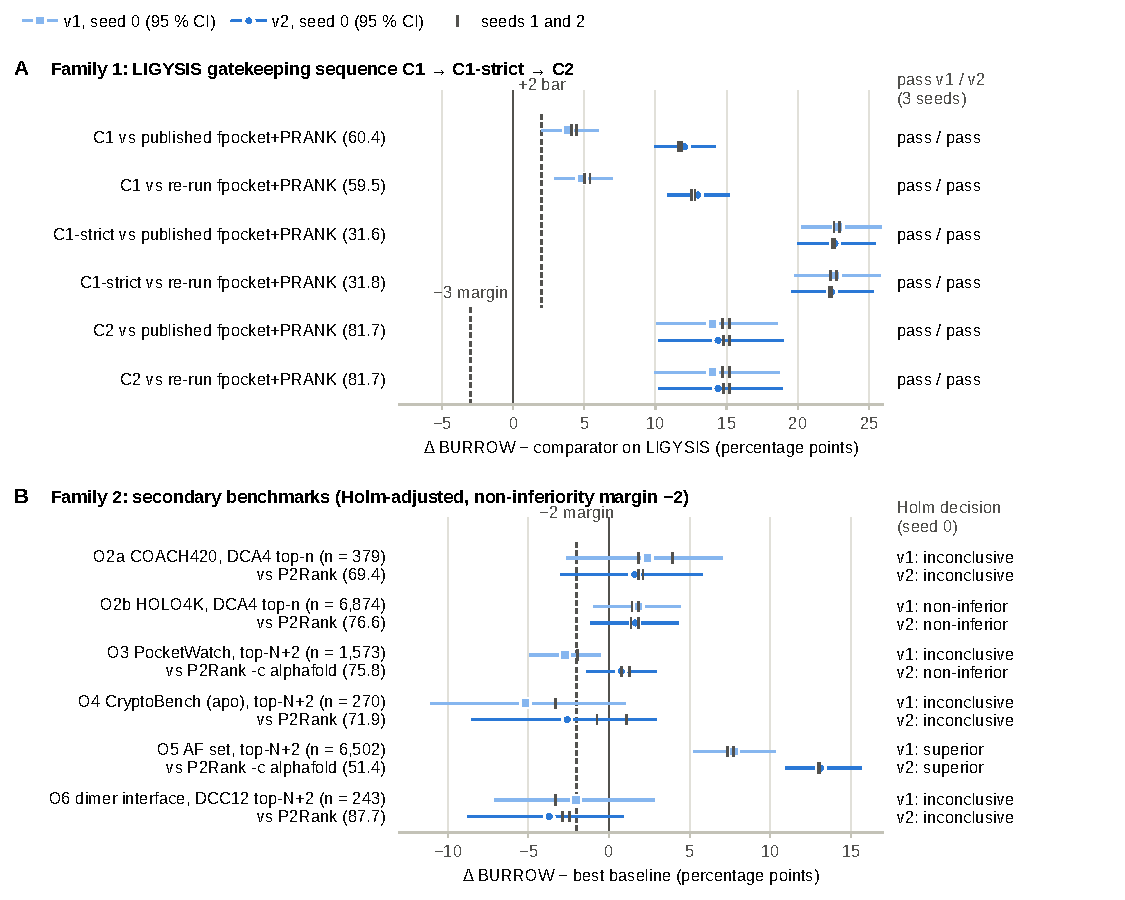
\includegraphics[width=\linewidth,height=0.55\textheight,keepaspectratio]{figures/fig3_prereg.pdf}\fi
\caption{{\bf Pre-registered test comparisons.}
Paired differences (BURROW minus comparator) for the two frozen versions, v1 (squares) and v2 (circles). Seed 0 is shown with 95\% paired cluster-bootstrap CIs (30\% sequence clusters, 1,000 resamples); ticks mark the point estimates of seeds 1 and 2. (A) Family 1, tested in a fixed sequence on LIGYSIS: C1, top-N+2 at DCC $\le$ 12 \AA{}; C1-strict, top-N+2 at DCA $\le$ 4 \AA{}; C2, pooled P1K. Comparators are the published fpocket+PRANK predictions and our re-run of fpocket 4.2.3 + PRANK 2.4.2 (comparator value in brackets). C1 required $\Delta$ $\ge$ +2 points with a CI above 0, and C1-strict required a CI above 0, for every seed and both comparators. C2 was a non-inferiority test at $-$3 (lower CI bound above $-$3). Each row group's criterion is printed at its left; dashed lines mark the +2 bar (C1 rows only) and the $-$3 margin (C2 rows only). (B) Family 2: non-inferiority with Holm correction (margin $-$2) against the better of P2Rank 2.5.1 and fpocket 4.2.3 + PRANK on identical inputs; ``superior'' means that the CI excludes 0. n, scored sites (ligands for COACH420 and HOLO4K). Right: pre-registered decisions.}
\label{fig3_prereg}
\end{figure}

\subsection*{Most of the LIGYSIS margin comes from ion sites and shorter output lists}

Two properties explain much of the LIGYSIS margin (Fig 4). First, 38\% of LIGYSIS sites (2,580 of 6,721) are ion sites (Fig 4C). For v2, the difference to our re-run of fpocket+PRANK was +29.5 points on ion sites, +4.7 [2.0, 7.7] on nucleotide and cofactor sites and +2.2 [0.1, 4.3] on other small molecules. The baselines were not trained on ions, which probably explains much of this gap. Without ion sites (4,141 sites, \texttt{small} ranker, post hoc), v2 led fpocket+PRANK by +3.0 to +3.5 points and P2Rank by +5.4 to +5.9 points; at 4 \AA{} the lead was +3.1 [1.5, 4.8] and +6.7 [5.2, 8.4]. v1 trailed fpocket+PRANK on these sites ($-$4.6 [$-$6.3, $-$2.9]).

\begin{figure}[!h]
\ifembedfigures\centering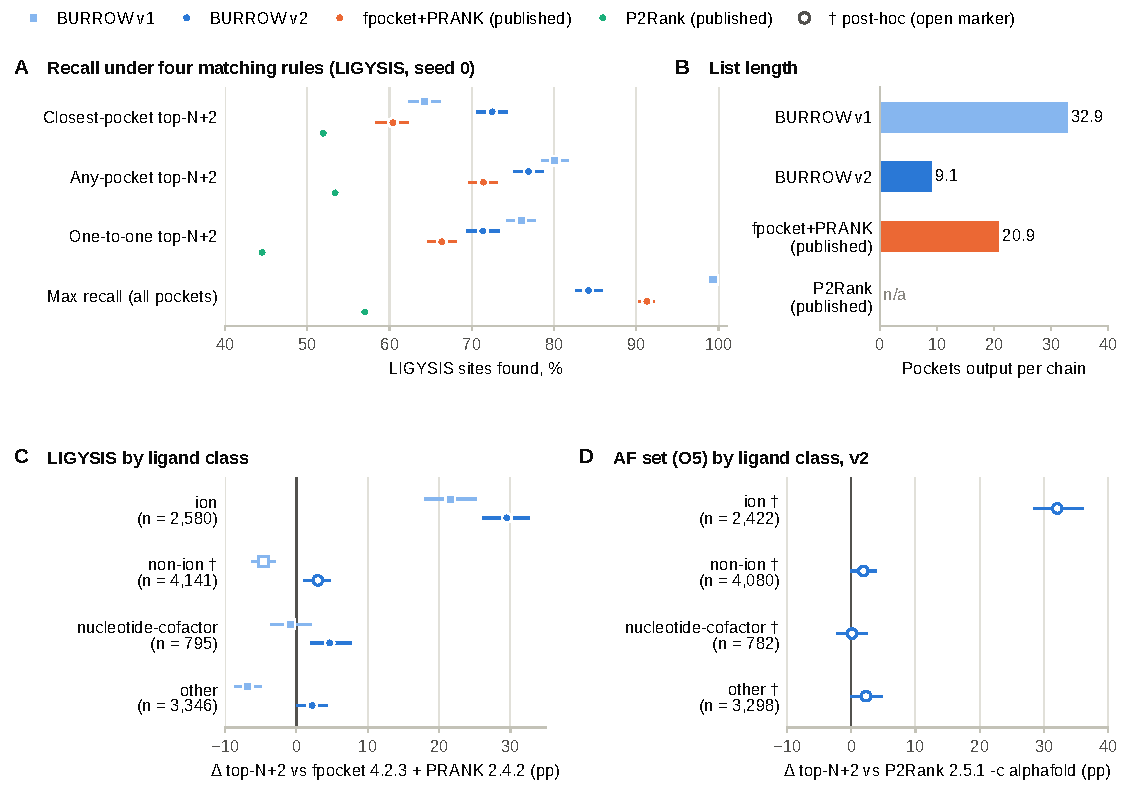
\includegraphics[width=\linewidth,height=0.55\textheight,keepaspectratio]{figures/fig4_composition_tradeoff.pdf}\fi
\caption{{\bf What drives the LIGYSIS margin: output length and ligand class.}
(A) LIGYSIS recall under four matching rules (seed 0). Closest-pocket top-N+2 is the LIGYSIS protocol (endpoint C1): a site is credited only to the pocket nearest to its centre. Any-pocket: any of the top N+2 pockets within 12 \AA{}. One-to-one: Hungarian matching of pockets to sites. Maximum recall: any pocket in the output. ``P2Rank (published)'' is the LIGYSIS authors' P2Rank prediction set; the text quotes our re-run of P2Rank 2.5.1 (52.6\%). Bars: 95\% cluster-bootstrap CIs (not computed for the published P2Rank predictions). (B) Mean number of pockets output per chain (not available for the published P2Rank predictions). The v2 output floor shortens the list. This raises closest-pocket top-N+2 and lowers coverage (any-pocket, one-to-one and maximum recall), so the C1 gain from v1 to v2 is an effect of output length rather than of better ranking. (C, D) Differences in top-N+2 by ligand class. (C) LIGYSIS ion, nucleotide-cofactor and other sites: pre-registered descriptive strata of C1 (\texttt{all} ranker) against our re-run of fpocket+PRANK. LIGYSIS non-ion (†, post hoc): the LIGYSIS site set without ions, with the \texttt{small} ranker. (D) AlphaFold set (†, post hoc, v2 only) against P2Rank's AlphaFold configuration; non-ion means nucleotide-cofactor plus other. Open markers: post-hoc analyses (not pre-registered). n, scored sites. Bars: 95\% paired cluster-bootstrap CIs.}
\label{fig4_composition_tradeoff}
\end{figure}

Second, the LIGYSIS protocol credits each site only to the pocket whose centre is closest to it. A low-ranked pocket that lies closer than the ranked hit therefore turns a hit into a miss, and long lists lose credit (Fig 4A and 4B). The agents found this on dev data (S3 Text). The v2 floor shortened the LIGYSIS list from 32.9 to 9.1 pockets per chain. C1 rose from 64.3\% to 72.5\%, while C1-strict (54.4\% to 54.2\%) and P1K (95.7\% to 96.1\%) did not change. Coverage fell: maximum recall from 99.3\% to 84.2\%, any-pocket top-N+2 from 80.1\% to 76.9\% and one-to-one top-N+2 from 76.0\% to 71.3\%. The v1-to-v2 gain is therefore an effect of output length, not of better ranking. The baselines ran with their default list lengths and might also gain from a tuned floor. C1-strict is robust to the floor but not to ligand class (+22.6 points overall, +3.1 on non-ion sites). \texttt{--min-score none} restores the v1 list exactly.

\subsection*{Runtime}

Fig 5 shows accuracy against runtime for the same 200 LIGYSIS chains, measured in one session. Run as one process (including start-up and file input and output), BURROW's default preset took 142 ms per structure, P2Rank 2.5.1 209 ms and fpocket 4.2.3 605 ms. Default BURROW is therefore about 1.5 times faster than P2Rank, short of the design target of 5 times. The optional fast preset, added after the test runs, took 48 ms (about 4.4 times faster than P2Rank) and cost 0.8 points of top-N+2 and 1.7 points of DCA4 recall on dev. On one warm core including parsing, the fast preset took 31.5 ms (about 6.6 times less than P2Rank's 209 ms, which includes Java start-up) and the default 99.2 ms. Only the fast preset met the design target of at most 70 ms per core; the default took 96.0 ms (median, excluding parsing). On 10,000 structures, three GPUs processed 411 structures per second with the default preset, against 171 for 24 CPU workers. The node was shared, so ratios carry about $\pm$30\% uncertainty. The CPU and GPU backends give output identical to the reference implementation (S3 Text).

\begin{figure}[!h]
\ifembedfigures\centering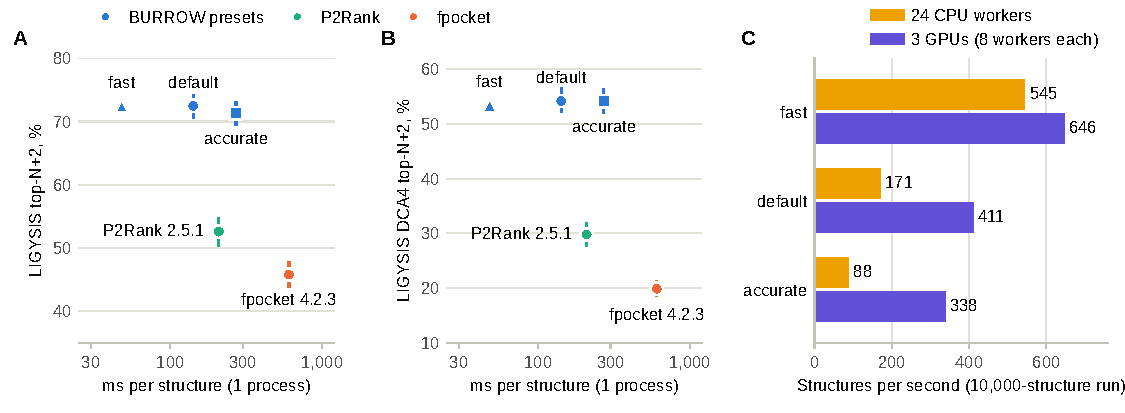
\includegraphics[width=\linewidth,height=0.55\textheight,keepaspectratio]{figures/fig5_speed.pdf}\fi
\caption{{\bf Accuracy and speed.}
(A, B) LIGYSIS top-N+2 (A) and DCA4 top-N+2 (B) against wall time per structure, from the final like-for-like timing. All tools ran in one session on the same 200 LIGYSIS chains, as a single process on one core (numerical libraries and P2Rank limited to one thread). Times are amortised and include process start-up, parsing and writing. P2Rank 2.5.1 runs in batch mode in one Java virtual machine; fpocket 4.2.3 runs one process per structure. Accuracy: BURROW v2 seed 0, \texttt{all} ranker, presets fast, default and accurate (fast was not pre-registered); P2Rank 2.5.1 and fpocket 4.2.3 alone (without PRANK rescoring) re-run on identical inputs. Bars: 95\% cluster-bootstrap CIs where computed (none for the fast preset). fpocket+PRANK is not shown because it was not timed in the final session. (C) Throughput of the BURROW command-line tool over 10,000 structures with 24 CPU workers, or with 3 GPUs and 8 CPU workers per GPU, including start-up, parsing and writing. The node was shared: other users' jobs ran at the same time.}
\label{fig5_speed}
\end{figure}

\subsection*{AlphaFold mode removes hallucinated pockets but is equivalent to a pLDDT filter}

In AlphaFold mode, BURROW removes terminal low-confidence segments and internal runs of 7 or more residues with pLDDT below 50, following AF2BIND ~\cite{gazizov2026}. It makes atoms with pLDDT below 80 partly transparent, down to full transparency at 40. The ranker is unchanged, and with uniform pLDDT of 90 or more the output is byte-identical to standard mode.

On the AlphaFold set (2,526 AFDB models, 6,502 sites), BURROW in AlphaFold mode reached 64.5\% top-N+2 recall against 51.4\% for P2Rank's AlphaFold configuration (Fig 6A). Again the gain came mostly from ion sites (+32.1 [28.3, 36.1]; non-ion +1.9 [$-$0.1, 3.9]; post hoc). Compared with the unmodified model, AlphaFold mode added +1.0 [0.1, 2.0] points and cut hallucinated top-N+2 pockets (mean pLDDT below 50, matching no site) from 2.80\% to 0.12\%. However, a simple filter that drops pockets with mean pLDDT below 70 ~\cite{carpenter2025,zillmer2025} was equally good (AlphaFold mode +0.4 [$-$0.5, 1.3]) and more precise (+2.4 points P1K), on dev as on test. The geometric mechanisms remove hallucinated pockets, as the filter does, and add no recall beyond it.

\begin{figure}[!h]
\ifembedfigures\centering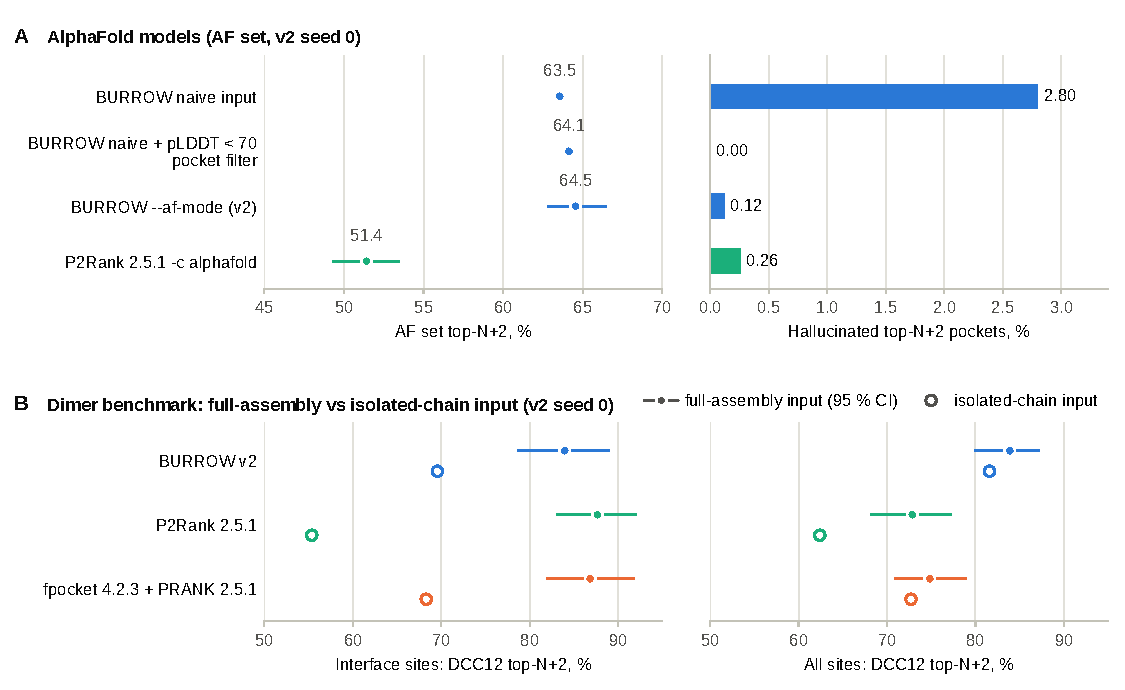
\includegraphics[width=\linewidth,height=0.55\textheight,keepaspectratio]{figures/fig6_af_dimers.pdf}\fi
\caption{{\bf AlphaFold models and protein dimers.}
(A) AlphaFold set (2,526 AlphaFold models, 6,502 sites, 1,691 cluster units). Left: top-N+2 (DCC $\le$ 12 \AA{}). Right: share of top-N+2 pockets that are hallucinated, that is, whose mean pLDDT is below 50 and that match no site within 12 \AA{} (pooled; no CI). BURROW rows: v2 \texttt{all} default model, seed 0, with naive input (no AlphaFold handling), with naive input followed by removal of pockets with mean pLDDT \textless{} 70, and in \texttt{--af-mode} (the pre-registered O5 variant). The naive and filter rows are descriptive and have CIs only for their paired differences to AlphaFold mode. Bars: 95\% cluster-bootstrap CIs. (B) Dimer benchmark (400 assemblies, 807 unique sites, of which 243 lie at an interface); the right-hand part shows recall over all sites. Filled markers: full-assembly input (site level, with 95\% CI). Open markers: every chain predicted alone. In this chain mode the unit is a chain copy, and a site is scored on each chain that carries it (634 interface rows and 1,678 rows in total), so the two input modes have different denominators. If a site counts as found when any isolated chain finds it, BURROW's interface DCC12 top-N+2 changes by $-$1.2 [$-$7.2, 4.4] points against assembly input (DCA4: $-$11.1 [$-$16.2, $-$5.6]). Rows for isolated chains are descriptive.}
\label{fig6_af_dimers}
\end{figure}

Precision on AlphaFold models was a weakness: P1K was 58.9\% against 73.9\% for P2Rank. An ablation model trained only on CHEN11 (251 P2Rank training structures, no ion labels) reached 78.2\%, which suggests, but does not show, that ion-heavy training lowers precision. An optional pLDDT-aware ranker raised P1K to 73.9\% but lowered PocketWatch top-N+2 by 3.4 and P1K by 14.6 points (descriptive; the advice to use it is test-informed). Two goals of the prompt were not met: PAE could not be downloaded (HTTP 403), and side-chain tolerance reduced dev recall ($-$10.9 points at an opacity factor $\lambda$ = 0.25) and is off. The AlphaFold set is holo-biased (median local C$\alpha$ RMSD to the PDB 0.38 \AA{}; only 95 benchmark sites, 89 scored, with mean pLDDT below 70).

\subsection*{Dimers: better on non-interface sites, not better on interface sites}

BURROW computes candidates, features and ranks on whole assemblies. The agents built a dimer benchmark from 400 PDB assemblies of LIGYSIS proteins (274 homomeric and 126 heteromeric, 2--8 chains), with symmetric copies merged and the same label-free merging of predictions for every method (Methods). With full-assembly input, BURROW recalled 84.0\% of interface sites against 87.7\% for P2Rank ($-$3.7 [$-$8.7, 0.9], inconclusive; hetero-interface $-$6.1, 66 sites; Fig 6B). It was far ahead on single-chain sites in assemblies (+19.0 [13.2, 25.9]) and over all sites (83.9\% against 72.9\%). Only 9 of the 243 interface sites are ion sites, so this endpoint is in effect a test on non-ion sites. With each chain given alone (descriptive, counted per chain copy), BURROW found 69.6\% of interface sites against 55.4\% for P2Rank (+14.2 [9.0, 20.1]). Counted per site, it lost only 1.2 points relative to assembly input at 12 \AA{} but 11.1 at 4 \AA{}, so the missing partner mostly reduces the precision of localisation. An interface-targeted cycle (v3) failed its gate (S1 Text). With 158 bootstrap units, CIs are about $\pm$5 points.

\subsection*{Apo and cryptic sites: not shown}

On CryptoBench apo structures, the v2 difference to P2Rank ranged from $-$2.6 to +1.1 across seeds, with CIs of about $\pm$6 points. BURROW had higher any-pocket recall (79.6\% against 74.8\%) and P1K (38.5\% against 30.1\%) but lower closest-pocket top-N. From holo to apo (233 paired sites), BURROW lost 10.7 points and P2Rank 7.7, so BURROW is, if anything, more sensitive to the apo state. At residue level it matched PocketMiner ~\cite{meller2023} on 35 apo chains (ROC-AUC 0.792 against 0.789; a small sample). Four apo-oriented training changes gave no dev gain (S1 Text). Allosteric sites were not evaluated.

\subsection*{Controls and ablations}

Controls support the main results (S1 Fig, S2 Fig). Shuffled training labels gave 35.9\% LIGYSIS top-N+2 ($-$28.4 against v1), about the level of one pocket at the protein centroid (37.0\%) and above evenly spaced surface pockets (18.3\%). Randomly shuffled ranks of BURROW's own pockets gave 14.6\% on dev. We also retrained BURROW without the training inputs that have a Foldseek TM-score of 0.5 or more to any test chain ~\cite{vankempen2024}, which removed 41\% of the 8,184 inputs (representative chains and assemblies). This changed 9 of 10 test rows by amounts within noise; the exception was COACH420 ($-$3.2 [$-$6.0, $-$0.3]). The gains on LIGYSIS and the AlphaFold set were largest for new folds (S1 Fig). No feature group was essential: the largest dev loss was 2.5 points, for metal features (single seed; the seed-to-seed standard deviation on dev is about 0.7 points). P2Rank retrained on 25\% of our training data (more exceeded the memory limit) was 6.7 points below stock P2Rank and 26.6 below BURROW v2 on LIGYSIS, but reached BURROW's level on HOLO4K and dimer interfaces. Our data alone therefore do not reproduce the largest gains, although this control is limited.

\subsection*{The agent-run process}

The project ran for about 22 h (14:54 on day 1 to 12:35 on day 2), including a 4.5 h pause caused by an API usage limit and the user's extension, and produced more than 130 git commits. The PI agent launched sub-agents for 25 project roles and 5 release and manuscript roles (Table 4) and logged 20 dated decisions (D0--D19). Independent agents caught errors that the producing agents had missed: residual training-set leakage that the builder's own check had passed (186 entries removed), a GPU threshold passed in single precision that changed outputs only at pLDDT exactly 70, a filter bug in one descriptive dimer table, and the fact that the v2 floor gained mainly by shortening lists. S2 Text lists all failure modes. The pause cost only wall-clock time, because long jobs ran in the background and wrote their state to disk.

\begin{table}[!ht]
\begin{adjustwidth}{-0.0in}{0in}
\centering
\caption{{\bf Agent roles.} Each row is one sub-agent role launched by the PI agent (Claude Code); roles 26--30 belong to the release and manuscript phase. Several roles were served by one long-lived agent that was resumed many times. Opus, Claude Opus 5.5; Sonnet, Claude Sonnet 5.5. S1 Table gives the full roster with outputs and checks.}
\label{table_agents}
{\footnotesize
\begin{tabular}{p{0.6cm}p{5.6cm}p{1.6cm}p{6.3cm}}
\hline
\textbf{\#} & \textbf{Role} & \textbf{Model} & \textbf{Main outputs} \\ \thickhline
-- & PI agent (one long session) & Opus & Design, pre-registration amendments, research tree and decision log, lessons, all commits \\ \hline
1 & Literature reviewer (with 2 research sub-agents) & Opus & Literature review \\ \hline
2 & Data acquisition & Opus & Dataset list with checksums and licenses; download and verification scripts \\ \hline
3 & Baselines engineer & Sonnet & P2Rank, fpocket+PRANK and 8 optional tools; all baseline runs; P2Rank retrained on our data \\ \hline
4 & Evaluation engineer & Opus & Metrics harness, LIGYSIS reproduction, cluster bootstrap, gated test runner and ledger \\ \hline
5 & Geometry and HPC engineer & Opus & Geometric primitives (CPU and GPU), exact fast backend, proteome run, ablations, speed \\ \hline
6--11 & Design reviewers, round 1 (external PI; prior work and data; statistics; algorithms and compute; AI-agent failure modes; biophysics and AlphaFold) & Opus $\times$6 & Six reviews \\ \hline
12--13 & Design reviewers, round 2 (external PI and statistics; data and agent risks) & Opus $\times$2 & Two reviews \\ \hline
14 & Training and dev set builder & Opus & Leakage-controlled BioLiP2 sets; apo counterparts \\ \hline
15 & AlphaFold test set and AlphaFold training labels & Opus & AlphaFold benchmark and labels \\ \hline
16 & Dimer benchmark builder & Opus & Dimer benchmark and evaluator \\ \hline
17 & Method developer & Opus & BURROW reference implementation, training, presets, v2 and v3 cycles \\ \hline
18 & AlphaFold-mode developer & Opus & AlphaFold-mode mechanisms, ablations, optional ranker \\ \hline
19 & Independent leakage auditor & Sonnet & Audit (found residual leakage; 186 entries removed) \\ \hline
20 & Independent dev-result reviewer & Opus & Review of dev results \\ \hline
21 & Independent test verifier (no project imports) & Opus & Recomputation of headline test numbers \\ \hline
22--23 & Process retrospectives & Sonnet $\times$2 & ``What should we stop doing?'' and ``what worked well?'' \\ \hline
24 & Report writer and number checker & Opus & Report; script that checks every reported number \\ \hline
25 & External report reviewer & Opus & Report review \\ \hline
26 & Release-repository builder & Opus & Release repository (scrubbed) \\ \hline
27 & Figure maker & Opus & Figures \\ \hline
28 & Manuscript writer & Opus & Manuscript and supporting texts \\ \hline
29 & Reference verifier & Opus & Verified bibliography \\ \hline
30 & Manuscript reviewer & Opus & Referee-style review of the draft \\ \hline
\end{tabular}}
\end{adjustwidth}
\end{table}

\section*{Discussion}

BURROW meets some goals of the prompt and misses others. On LIGYSIS it passed all three pre-registered tests against fpocket+PRANK, the best published method: superiority in recall at 12 \AA{} and at 4 \AA{}, and non-inferiority in precision (whose CI also excluded zero). Comparisons with other published methods are descriptive. BURROW is non-inferior on HOLO4K and PocketWatch and superior on the AlphaFold set. It does not show better generalisation to apo or cryptic sites, it is not better at dimer interfaces, and allosteric sites were not tested. AlphaFold mode removes hallucinated pockets but adds nothing over a pLDDT filter, and PAE was not used. The default preset missed both speed targets of the design: at most 70 ms per core (median 96 ms) and at least 5 times faster than P2Rank (about 1.5 times per process). Only the fast preset, added after the test runs, met the first.

Two qualifications apply to the LIGYSIS margin. Ion sites make up 38\% of LIGYSIS, and on them BURROW gains about 30 points, probably because the baselines were not trained on ions; on non-ion sites the margin over fpocket+PRANK is +3.0 to +3.5 points. Output length is the second: the v2 floor raised C1 by 8.2 points while C1-strict and P1K did not change, and the baselines were not given a tuned floor. The localisation margin (DCA4 +22.6 points) is robust to the floor but not to ligand class: without ion sites it is +3.1 [1.5, 4.8] against fpocket+PRANK and +6.7 [5.2, 8.4] against P2Rank. The clearest non-ion gain is therefore over P2Rank. The LIGYSIS protocol also judges interface sites on a single chain, and its 12 \AA{} criterion is lenient; on dev, the median distance between a successful BURROW pocket and the site centre is 3.3 \AA{}, against 4.7 \AA{} for P2Rank.

Where does the gain come from? Before the floor, the LIGYSIS candidate set has 99.3\% maximum recall at 32.9 pockets per chain, against 57.7\% for P2Rank at about 5 (fpocket reaches 91\% at 20.9). Candidates alone are not enough, because geometry-only ranking is at P2Rank's level. With the same ranker, BURROW's candidates gave 16.5 points more DCA4 recall on dev than fpocket's. Both parts are needed, as the literature analysis suggested ~\cite{utges2024}. Fold-disjoint retraining is evidence against memorisation of folds, but training labels built like LIGYSIS sites may favour BURROW on LIGYSIS over benchmarks with other site definitions.

Several decisions shaped the results (Table 5). The weakest point is the timing of v2. The floor was derived on training and dev data and adopted before any v1 test score was computed, but v1 prediction files had existed for 70 minutes. The independent verifier could not rule out that they had been inspected, and the session transcripts are not archived, so this cannot be checked. The pre-registered claims hold for v1 alone, which limits the damage; ideally, the policy on list length would have been fixed before the first test run. Other test-informed steps were disclosed: the v3 cycle was motivated by a test result (and changed nothing), and the advice to use the AlphaFold ranker relies on descriptive test rows. No default was switched on test evidence; for example, the fast preset was better on CryptoBench test data (+6.7 points), but the default was kept.

\begin{table}[!ht]
\begin{adjustwidth}{-0.0in}{0in}
\centering
\caption{{\bf Decisions that affect how the results should be read.} D numbers refer to the decision log in the project's research tree. Each entry gives what was decided, why, and the consequence for interpretation.}
\label{table_decisions}
{\footnotesize
\begin{tabular}{p{3.2cm}p{5.7cm}p{5.8cm}}
\hline
\textbf{Decision} & \textbf{Reason} & \textbf{Consequence} \\ \thickhline
Ions included in the headline model (D1) & LIGYSIS and the published bar include ion sites; metal sites are common and poorly covered by surface-point methods & Ion sites carry much of the C1 margin; a pre-registered \texttt{small} ranker and post-hoc ion-free analyses separate the effect \\ \hline
Two rankers, mapped to benchmarks by ligand definition (D1) & Benchmarks differ in whether ions count; mapping fixed before results & Fair comparison on ion-free benchmarks; two models to maintain \\ \hline
LIGYSIS-style training labels from BioLiP2 (D1) & Train on the same site definition as the main benchmark; keep all 2,775 LIGYSIS chains for comparability & May favour LIGYSIS over benchmarks with other site definitions \\ \hline
Conservative leakage fix (D6) & Independent audit found residual leakage; all 186 flagged entries removed, not only the 8 hard failures & Smaller training set; no full re-audit after the fix \\ \hline
Accept failure of the candidate-recall gate G1 (D7) & Gate failed on dev (58.6\% vs 88\% at $\le$ 40 geometric candidates); the pre-specified fallback (fpocket candidates) was worse & Deviation from the design, disclosed; own candidates kept \\ \hline
Speed budget (D5): default $\le$ about 100 ms per core, at least 5 times faster than P2Rank & Speed was a goal of the prompt & Default: 96 ms median per core, about 1.5 times faster than P2Rank per process; the 5-fold target was missed; the fast preset was added later \\ \hline
Suppression radius 10 \AA{} (D7) & Chosen by one-to-one P1K on cross-validation; 12--14 \AA{} would raise top-N+2 by spreading pockets & Avoids tuning to the 12 \AA{} tolerance of the metric \\ \hline
Output floor adopted as v2 before scoring v1 (D12, D13) & Dev evidence that the closest-pocket rule gives less credit to long lists; $\tau$ chosen on training-set cross-validation & Adopted 70 min after v1 test predictions existed; v1 also reported and passes alone; C1 gain is an output-length effect \\ \hline
AlphaFold mode = pruning and soft occlusion with the standard ranker; AlphaFold ranker optional (D8) & The AlphaFold ranker lost recall near disorder on dev & Default unchanged; \texttt{--af-ranker} recommended only for AFDB screening (test-informed) \\ \hline
v3 interface cycle with a fixed gate (D14, D15) & Motivated by the O6 test result (test-informed, disclosed) & Gate failed; nothing changed \\ \hline
No further test version (D16) & Three dev cycles showed saturation on non-ion ranking & Remaining time used for checks, descriptive rows and reviews \\ \hline
No default switched on test evidence (D18, D19) & Fast preset and per-region floor evaluated as options only & Fast preset looked better on some test rows but the default was kept \\ \hline
\end{tabular}}
\end{adjustwidth}
\end{table}

The agents followed rules that a careful human group would follow: reproduce published numbers first, pre-register, audit data independently, use controls and report negative results (S1 Text). Applying them caught real errors. The weaknesses were ones that also occur in human projects under time pressure: claims were fixed before the benchmark had been broken down by ligand class, the policy on list length was decided after the first test predictions existed, some branches were explored past the point of diminishing returns, and the agents' self-reports needed independent checks. Human oversight would be most useful when the claims are fixed, when a test result is first seen, and when deciding how strongly to state a result. This was a single run of one agent system on one task, without repetition or comparison with a human team, so we cannot say how often such a run succeeds.

Open follow-ups are a pre-registered, tuned output floor for the baselines (the most direct test of the output-length caveat), a context-dependent floor (on dev, 65\% of v2's non-ion misses were pockets that the global floor removed), a larger interface benchmark with more multimer training data, cheap flexibility models for apo sites, PAE through bulk download, and timing on an exclusive node.

\section*{Materials and methods}

\subsection*{Agent-based project execution}

\textbf{Setup.} The project ran on 26--27 October 2026 on one shared node (64-core AMD EPYC 9554, four RTX 4090 GPUs, an effective memory cap of about 79 GB) in a Singularity container on the ETH Euler cluster, with read-only copies of the PDB ~\cite{berman2000} and the AlphaFold database ~\cite{varadi2022}. The agents used Claude Code with Claude Opus 5.5 and Claude Sonnet 5.5; the Claude Code version, tool settings and token usage were not recorded. The prompt (S2 Text) set the goals, a 24 h budget, the hardware and process rules: design through independent critique, review of every result by an agent that did not produce it, a research tree as memory, a lessons file, and end-to-end reproducibility.

\textbf{Roles.} One PI agent (Opus, one long session) planned, delegated, reviewed and integrated. It owned the design, the pre-registration amendments, the research tree with its decision log, the lessons file and all git commits, and it did not write method code. Each sub-agent was a fresh Claude Code agent launched with a written brief (goal, owned files, deliverables, rules) and could be resumed with follow-up messages; several roles were served by one long-lived agent resumed many times (for example the evaluation engineer, the method developer and the geometry and HPC engineer). Table 4 lists the 30 roles; the literature reviewer also used two research sub-agents. Opus served most roles, and Sonnet the baselines engineer, the leakage auditor and the process retrospectives. Agent briefs and session transcripts were not archived, so individual delegation steps cannot be audited. After the prompt, the human sent four messages (S2 Text); the environment twice restarted the session with an empty ``Continue'' message.

\textbf{Design by critique.} A literature agent reviewed methods, benchmarks and metrics. Six independent reviewer agents assessed the PI's first design (external PI; prior work and data; statistics; algorithms and compute; AI-agent failure modes; biophysics and AlphaFold), and two assessed the second. Each proposed concrete changes or stated that none were needed. Reviews were capped at two rounds, although the prompt allowed three.

\textbf{Independence and gating.} Four checks were done by agents that had not produced the checked work: the leakage audit (re-implemented from scratch), the review of dev results, the recomputation of headline test numbers (without project code, with the LIGYSIS authors' code for C1) and the review of the report. The method, the dimer evaluator and the benchmarks were not re-implemented. A script checks each of the 1,724 tagged numbers in the project report against committed result files. Test sets could be scored only through a gated script that refuses modified files, records model checksums and appends to a test ledger, with at most three frozen versions. Predictions for frozen versions were generated from isolated git worktrees. Each agent owned a list of files, and only the PI committed.

\textbf{Interruptions and lessons.} The session restarted twice in the first two hours, and an API usage limit paused all agents for about 4.5 h. Long jobs ran detached with logs and completion markers, and agents were resumed from their files, so no work was lost. Two fresh agents ran process retrospectives, and the PI condensed the lessons into 15 rules (S2 Text).

\textbf{Manuscript.} A sub-agent wrote this manuscript from the verified report and result files, applying a writing guide based on Clark, Martin and Mahowald ~\cite{clark2026} (``edit-for-clarity''); another made the figures with a plotting guide (``dataviz''), reading each value from a committed result file. Other sub-agents checked the references against Crossref and PubMed, reviewed the draft as a referee, and built the release repository. Every number in the text was checked by script against the project report and result files.

\subsection*{Method}

S3 Text gives the full specification; the key parameters are as follows. BURROW reads PDB or mmCIF files with gemmi ~\cite{wojdyr2022} and keeps protein heavy atoms, so predictions do not depend on HETATM records (tested). Grid points (1 \AA{}) lie at least the van der Waals radius plus 1 \AA{} from every atom and within 6 \AA{} of the nearest atom. Points with a LIGSITE count (7 directions, 8 \AA{}) of 2 or more are kept at full resolution, the rest on a 3 \AA{} sub-lattice ~\cite{hendlich1997}. Metal candidates lie 1.95--2.35 \AA{} from a side-chain atom that can coordinate a metal, with at least two coordinating atoms within 2.6 \AA{} and no other atom closer than 2.4 \AA{}. Thirty Fibonacci rays (60 in the accurate preset) are marched through the full-atom and backbone-plus-C$\beta$ grids to 6, 10 and 16 \AA{} (plus 24 \AA{}). With local counts, weighted contact number, protrusion and metal geometry, this gives 84 features (86).

The point scorer is a LightGBM classifier ~\cite{ke2017} (250 trees, 63 leaves). A point is positive if it lies within 4 \AA{} of a non-ion ligand atom or, for the \texttt{all} ranker, within 3 \AA{} of an ion. Pockets are formed by single linkage at 2.05 \AA{} over several thresholds of buriedness and point score, with splitting of long components. The pocket ranker (LightGBM, 300 trees, 15 leaves, 76 descriptors) is trained with cross-entropy on cross-fitted point scores (5 folds of 30\% sequence clusters) and the target clip(1 $-$ q/12, 0, 1), where q is the smallest DCC to a site whose ligand atoms lie within 4 \AA{} of the pocket centre. Suppression removes pockets within 10 \AA{} of a kept pocket, with a residue Jaccard index of 0.75 or more, or with point overlap of 0.3 or more; at most 50 are kept. The v2 floor ($\tau$ = 0.03, at least three kept) was chosen by cross-validation over training-set clusters under the condition that closest-pocket recall, DCA4 recall, one-to-one P1K and top-N must not decrease. Gradient-boosted trees were chosen because they are fast on tabular features and because the prompt warned that large deep-learning models overfit. Most hyperparameters were set in early runs on the P2Rank training sets (CHEN11 and JOINED) and chosen among about ten settings on dev under the speed budget (decision D5), so dev numbers are somewhat optimistic; test sets were not used for any choice.

The default preset (30 rays, 3 \AA{} sub-lattice, only points with buriedness of at least 0.7 and metal candidates scored) was used for all pre-registered claims. The accurate preset (60 rays, 2 \AA{} sub-lattice) is shipped because it was more than 1 point better on non-ion dev sites. The fast preset (1.5 \AA{} grid, 12 rays, 100 trees of 31 leaves) was added after the test runs, selected on training-set cross-validation by a rule fixed in advance (at most 35 ms and a 2-point loss) and confirmed once on dev. \texttt{--af-mode} reads pLDDT from the B-factor column, removes low-confidence segments ~\cite{gazizov2026} and gives the remaining atoms an opacity w = clip((pLDDT $-$ 40)/40, 0, 1); \texttt{--af-ranker} optionally adds pocket pLDDT descriptors. Multimers need no special mode: all chains enter the grids, features and ranker. The reference implementation uses NumPy ~\cite{harris2020} and SciPy ~\cite{virtanen2020}; the fast backend uses Numba on the CPU ~\cite{lam2015} and Triton/PyTorch kernels on the GPU ~\cite{tillet2019,paszke2019}. Both give output identical to the reference (S3 Text).

\subsection*{Training and development data}

Training data came from BioLiP2 (snapshot 2025-11-12) ~\cite{zhang2024}: X-ray or EM structures at 3.0 \AA{} or better, receptor chains of at least 50 residues and BioLiP2's relevant ligands, including metal ions. The union of all test sets was frozen and checksummed before the training build. A training chain was removed if MMseqs2 ~\cite{steinegger2017} found a hit to the test union with E \textless{} 10$^{-3}$ and at least 30\% identity over at least 50\% coverage or 80 aligned residues, or if it shared a PDB ID or UniProt accession with a test entry. This removed 77.4\% of BioLiP2 chains. Sites were built in the LIGYSIS style ~\cite{utges2024}: ligands from up to 20 entries per UniProt accession were superposed onto a representative chain and clustered by binding-residue fingerprints. Dev data were 10\% of sequence clusters, built the same way. The independent audit found residual leakage (8 hard failures); the agents removed every entry that any tier of the audit flagged (186 entries, 2.6\%), which left 6,475 training and 579 dev chains (8,184 training inputs including assemblies). Before this fix, the training set had 14,073 sites, 37.7\% of them ion-only. No full re-audit was run afterwards; the test verifier later found none of the 2,565 LIGYSIS UniProt accessions in training or dev data. S3 Text gives the full construction.

\subsection*{Benchmarks, baselines and statistics}

Table 2 lists the benchmarks and S3 Text their construction. LIGYSIS was scored with the authors' representative chains and redundancy filter ~\cite{utges2024}. COACH420 and HOLO4K were scored with P2Rank's rules on the explicit relevant-ligand versions ~\cite{krivak2018}; our evaluator reproduced P2Rank's own to 0.1\%. The AlphaFold set maps LIGYSIS sites onto AFDB v6 models by UniProt numbering. The dimer set uses assembly 1 of LIGYSIS proteins (2--8 chains); a site is at an interface if 3 or more residues on each of 2 or more chains contact it, and symmetric copies and every method's predictions are merged at a residue-set Jaccard index of 0.5 or more. scPDB ~\cite{desaphy2015} was not used as a test set (no stated license, one site per entry, overlap with LIGYSIS), nor were AF2BIND (residue-level, about 65 test chains) and HOTPocket (a catalogue of predictions). Comparators were run on identical, cleaned inputs: P2Rank 2.5.1 (default, and its AlphaFold configuration on predicted structures) ~\cite{krivak2018} and fpocket 4.2.3 rescored by PRANK ~\cite{leguilloux2009,krivak2015} (PRANK 2.4.2 on LIGYSIS, as in the original paper; both versions gave identical LIGYSIS numbers). Published deep-learning predictions on LIGYSIS and our runs of other tools are descriptive (S1 Text).

The bootstrap resampled sequence clusters (30\% identity) 1,000 times with a fixed seed; differences are paired, failures count as misses, and P1K is recomputed in each resample. Family 1 had three requirements, each for every seed and both comparators: for C1, $\Delta$ $\ge$ +2 points with CI \textgreater{} 0; for C1-strict, CI \textgreater{} 0; and for C2, a lower CI bound above $-$3. Family 2 used a margin of $-$2 points against the better of P2Rank and fpocket+PRANK, with Holm correction over six endpoints ~\cite{holm1979}. Strata were pre-registered as descriptive; analyses labelled post hoc were added after the test runs. The pre-registered sensitivity analysis on the common chain subset was run (C1, v2 seed 0: +11.8 [9.7, 13.8] on 6,700 sites); the one with UniProt bootstrap units was not. The pre-registration was frozen at 15:39 CET on day 1 (git time); amendments A1 (dimer copy grouping), A2 (ligand placement for C1-strict) and A3 (fpocket 4.2.3 for the reproduction gate) each preceded the relevant predictions. The planned v3 and a later per-region floor (v3b) failed their dev gates, so v2 is final; twelve models (3 seeds $\times$ 2 rankers $\times$ 2 presets) were frozen per version.

\subsection*{Data availability}

Code, trained models, predictions on all test sets, the data underlying every figure and the scripts that regenerate every table are available at \url{https://github.com/<to-be-published>/burrow} [repository URL to be completed by the authors]; an archived copy with a DOI will be minted at publication [DOI to be completed]. Raw data come from public sources: the PDB, the AlphaFold database (v6), BioLiP2, LIGYSIS (Zenodo 10.5281/zenodo.13121414), the P2Rank datasets (COACH420, HOLO4K), CryptoBench, PocketMiner and PocketWatch. The repository lists the version, checksum and license of each dataset; restricted or very large data are not redistributed, but download scripts and manifests are provided. No human or animal data were used.

\section*{Supporting information}

\paragraph*{S1 Text.}
\label{S1_Text}
{\bf Methods that did not work.} Every major negative or abandoned approach, with what was tried, the evidence and the lesson.

\paragraph*{S2 Text.}
\label{S2_Text}
{\bf Agent setup and prompts.} Details of the agent setup, the verbatim project prompt and the verbatim follow-up messages.

\paragraph*{S3 Text.}
\label{S3_Text}
{\bf Extended methods and results.} Full technical specification of BURROW, the training data, the benchmarks and the statistics, and longer versions of several Results paragraphs.

\paragraph*{S1 Table.}
\label{S1_Table}
{\bf Agent roster.} All sub-agent roles with model, inputs, outputs and the independent checks that each role performed.

\paragraph*{S1 Fig.}
\label{S1_Fig}
{\bf Differences by fold novelty.} Differences (BURROW minus comparator, percentage points; seed 0, default preset) in each benchmark's endpoint metric, stratified by the maximum Foldseek TM-score between the test structure and any training structure (\textless{} 0.5, novel fold). Comparators as in the pre-registered endpoints: (A) LIGYSIS top-N+2 against fpocket 4.2.3 + PRANK 2.4.2; (B) AlphaFold set top-N+2 against P2Rank 2.5.1 in its AlphaFold configuration; (C) dimer interface DCC12 top-N+2 against P2Rank 2.5.1, recomputed post hoc (†, open markers) on the 243 interface sites only, because a filter bug had made the original fold strata use all dimer sites (descriptive only; v2 only); (D) HOLO4K DCA4 top-n; (E) PocketWatch top-N+2; (F) CryptoBench (apo) top-N+2. n, sites (ligands for HOLO4K) per stratum; *, fewer than 100. Bars: 95\% paired cluster-bootstrap CIs. Strata are descriptive.

\paragraph*{S2 Fig.}
\label{S2_Fig}
{\bf Ablations and controls.} Paired differences (ablation minus reference, percentage points) with 95\% paired cluster-bootstrap CIs (1,000 resamples; BioLiP2 dev and test sets: 30\% sequence clusters; apo-dev: UniProt units). In A and B, values beyond the axis are drawn as arrows with the value and CI printed. (A, B) Development sets. Models were trained with the frozen v1 recipe (seed 0) and paired against the v1 seed-0 model of the same ranker (filled: \texttt{all}; open: \texttt{small}); metric DCC12 top-N+2. A1: training entries with Foldseek TM-score $\ge$ 0.5 to any test chain removed. A2: trained on the CHEN11 structures only. A3: point labels and pocket targets permuted within each protein (negative control). A4: one feature group removed from the point model, together with the matching pocket descriptors from the ranker. (C, D) Test sets (descriptive; not part of the pre-registered families), in each benchmark's endpoint metric (DCA4 rows: DCA $\le$ 4 \AA{} top-N+2; dimer: interface DCC12 top-N+2). (C) A1 against v1, and A1 retrained with the v2 output floor against v2. (D) A2 and A3 against v1, on a wider axis.

\section*{Acknowledgments}

We thank the authors of LIGYSIS, P2Rank, fpocket, CryptoBench, PocketWatch, BioLiP2 and the AlphaFold database for making their data and code public. The LIGYSIS authors' published predictions and evaluation code made the reproduction gate possible.

\section*{Author contributions}

[Author contributions (CRediT roles) to be completed by the submitting authors. AI-agent contributions are described in the box at the start of the article, in Methods (``Agent-based project execution'') and in S2 Text.]

\section*{Funding}

[Funding statement to be completed by the submitting authors.]

\section*{Competing interests}

[Competing interests statement to be completed by the submitting authors.]

\nolinenumbers
\bibliography{references}

\end{document}
